% -------------------------------------------------------------
% Arquivo :  relatório modelo
% -------------------------------------------------------------
% O percentual(%) serve para incluir comentários:
% tudo o que fica à direita dele não é interpretado pelo LaTex
% Linhas e espaços em branco também **NÃO** são
% interpretadas pelo LaTex

%% As intruções seguintes são o cabeçalho e devem estar antes do
%% \begin{document}

%\documenclass: mandatorio, indica o tipo/formato de documento
\documentclass[brazilian,12pt,a4paper,final]{article}
% tamanhos de fontes: 10pt, 11pt ou 12pt
% opções de estilo (padrões): article, report, book, slide, letter (artigo, relatorio, livro, apresentação de slides, carta)




%% Pacotes extras (opcionais):

% *babel* contem as regras de ifenização
\usepackage[brazil]{babel}

% *t1enc* permite o reconhecimento dos acentos inseridos com o teclado
%\usepackage{t1enc}

% *inputenc* com opção *utf8* permite reconhecimento dos caracteres com codificação UTF8, que é padrão dos esditores de texto no Linux. Isso permite reconhecimento automático de acentuação.
\usepackage[utf8]{inputenc}


% *graphicx* é para incluir figuras em formato eps
\usepackage{graphicx} % para produzir PDF diretamente reescrever esta linha assim: \usepackage[pdftex]{graphicx}

% *color* fontes soloridas
\usepackage{color}
%%% fim do cabecalho %%%

\pagestyle{empty}
\title{Trabalho sobre Integração Numérica}
\author{Aluno: Leonardo Machado Barcelos - Matrícula: 00302060 \\ IF-UFRGS}

\begin{document}
\maketitle
\begin{abstract}
O presente trabalho tem por objetivo a comparação da convergência do erro associado à
integração numérica utilizando os Métodos de Simpson e do Trapézio. Chegou-se a conclusão de
que que o erro do método de Simpson converge mais rápido para zero do que o do Trapézio.
% as quebras de linha coma a de cima não são interpretadas
% para forzar quebra de linha deve ser deixada uma linha em branco
\end{abstract}

%Abaixo podem ver como se deve colocar letras acentuadas ou latinas se
%o pacote *t1enc* não dfosse usado
\section{Introdu\c{c}\~ao}
% Aqui a Introdução \c{c} e \~a  é a forma standar  de escrever
% carateres ASCII extendidos (acentos, etc), porem com o pacote t1enc
% declarado acima podemos escrever diretamente ç em lugar d \c{c}, etc
Para testar os dois métodos, foi utilizada uma função que não tem primitiva:
$$ \int_{0}^{1} e^{-x^2}\sqrt{1-x^2} dx $$
Para ambos os métodos, foram calculadas as integrais variando o número de divisões do intervalo
a ser integrado de dois em dois, começando com duas divisões. Conforme o número de divisões vai
aumentando, o erro tende a diminuir. A seguir serão mostrados gráficos de comparação das
convergências dos erros de cada método.
\section{Método de Simpson}
\begin{center}
    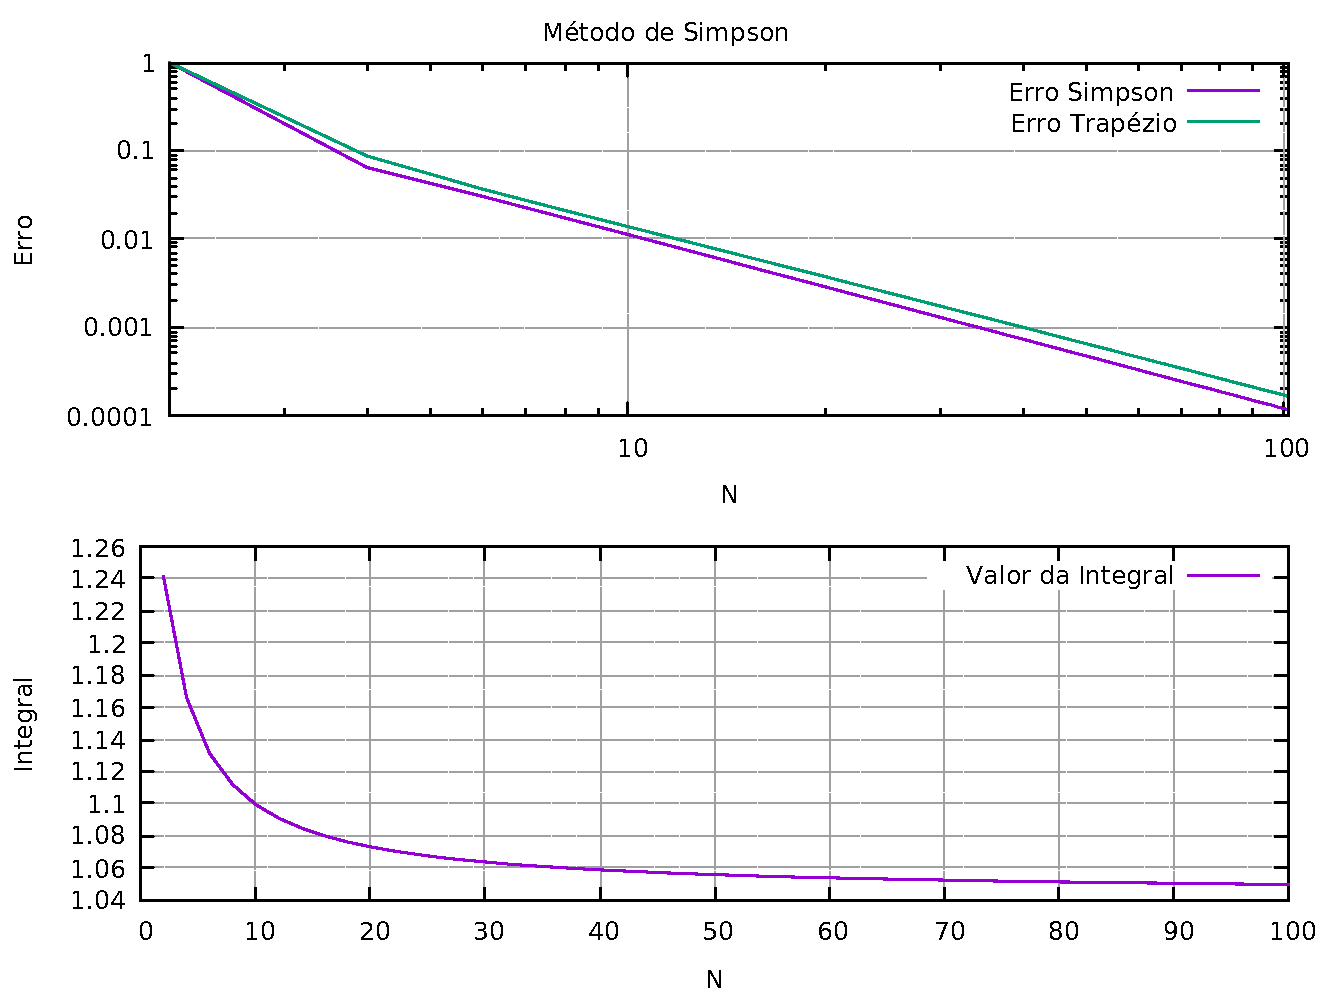
\includegraphics[width=12cm]{simpson.pdf}
\end{center}
Como é possível verificar na figura anterior, o primeiro gráfico é um comparativo entre
a convergência do erro do Método de Simpson e do Trapézio. De acordo com o gráfico, o erro
do método de Simpson converge mais rápido.

\section{Método do Trapézio}
\begin{center}
    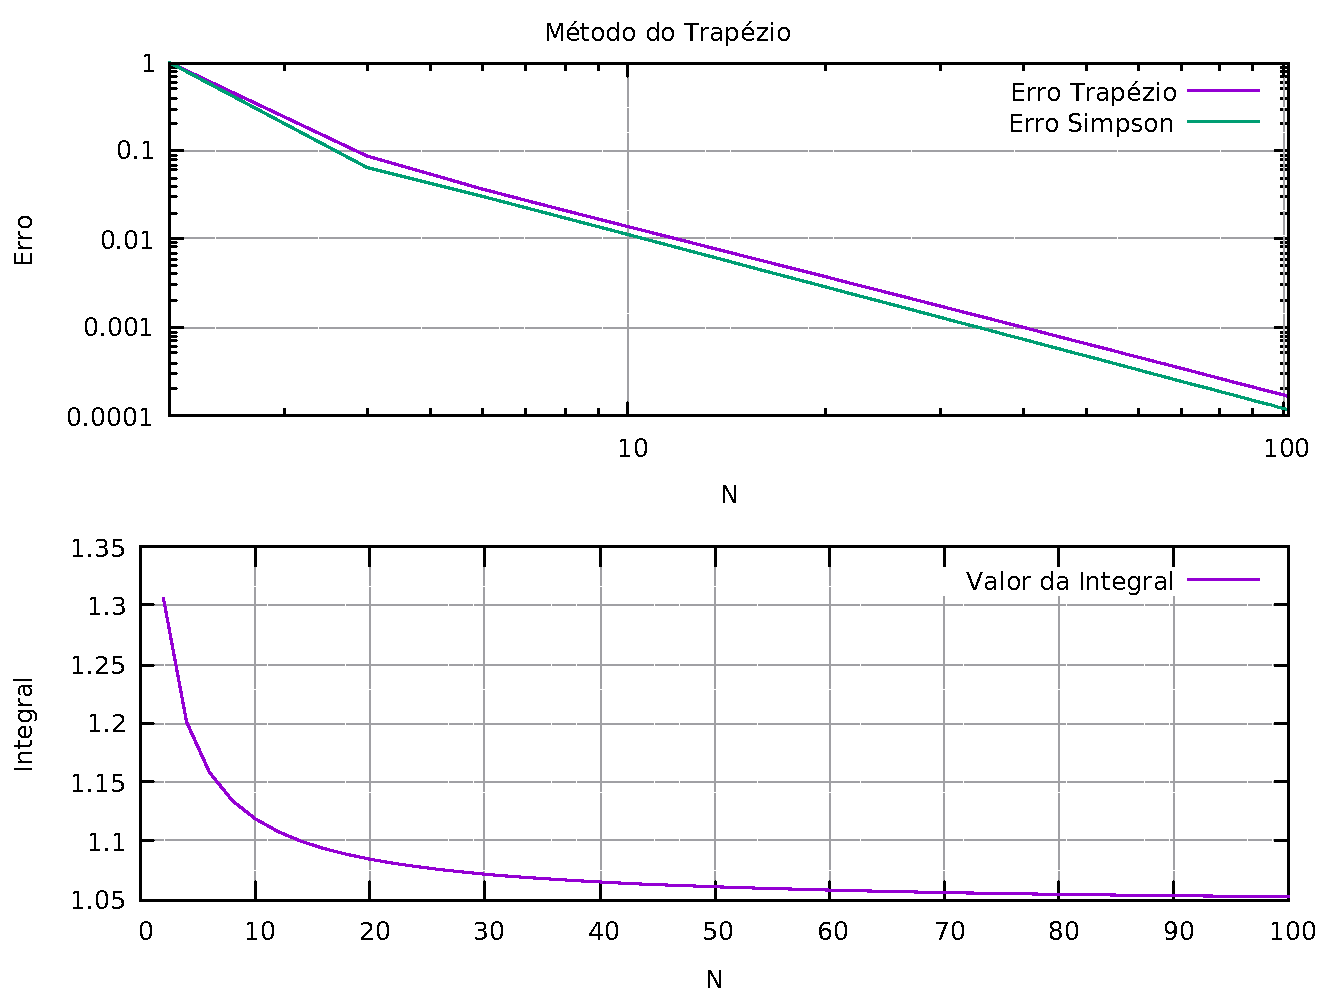
\includegraphics[width=12cm]{trap.pdf}
\end{center}
Na figura anterior, é o mesmo comparativo, porém no gráfico mais abaixo é apresentada a
convergência do valor da integral no intevalo $[0,1]$.

\section{Conclusões}
Portanto, pode-se concluir que o método de Simpson converge para o valor correto da integral
mais rapidamente, ou seja, o seu erro vai pra zero mais rapidamente.

\end{document}

